\subsection{Les notifications}

Durant l'utilisation de l'application, des notifications sont utilisées pour faire passer des messages de jeu aux joueurs. A chacun de ces événements, une notification s'ajoute sur l'écran puis disparaît après une certaine durée. L'application gère aussi les multiples notifications avec un empileur de notifications. La notification la plus récente s'affichera en dessous de l'ancienne plus récente. \\

L'empileur de notification est une liste de notifications qui commence vide et une notification s'y ajoute lorsque que cela est voulu. A partir du moment où la première notfication est ajoutée, un timer est activé afin d'effacer la notification après la durée prédéterminée. Le timer est stoppé lorsque l'empileur est vide pour que lorsqu'une première notification s'ajoute, elle ne disparaisse pas parce qu'elle a été ajoutée juste avant la fin de la durée. A chaque événement produit par le timer, les notifications sont remontées vers le haut afin de garder l'ordre d'apparition des notifications. Ainsi, nous évitons des superpositions de notifications ou des mélanges de position entre les anciennes ou récentes notifications.

\begin{figure}[h!]
	\centering
	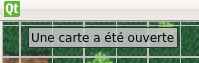
\includegraphics[width=0.5\textwidth]{img/notification.png}
	\caption{Notification lors de l'ouverture d'une carte}
	\label{fig:notification}
\end{figure}